\documentclass[expanded]{lkx_pset}

\title{CS181 Problem Set 3}
\author{Lev Kruglyak}
\due{March 10, 2024}

\usepackage{pgfplots}
\pgfplotsset{compat=1.14}
\usepackage[outputdir=build]{minted}
\usepackage{graphicx}


\collaborator{AJ LaMotta}

\begin{document}
\maketitle

\begin{problem}{1}[Connecting Bayesian and Frequentist Approaches]
\end{problem}

\begin{solution}
	You observe a fixed number \(N\) of coin flips (either
	heads or tails) of which \(Y\) (a random variable) are heads. You assume that these are drawn by flipping a coin with an unknown probability \(\theta\) of
	landing heads. That is, we choose a \textbf{Binomial likelihood}
	\(Y \sim \mathrm{Bin}(N, \theta)\).

	The PMF of this distribution is given by
	\[
		p(Y=y) = {\binom{N}{y}} \theta^{y} (1-\theta)^{N-y}.
	\]
	\begin{part}{1}[Frequentist paradigm and MLE]
	\end{part}
	\begin{parts}
		\begin{part}{}
			The (log) likelihood is all we need for frequentist inference. Derive the MLE estimate for \(\theta\) given the observations \(Y = y\). That is, find \[\arg \max_{\theta} \log p(Y = y \mid \theta).\]
		\end{part}

		Computing the log likelihood, we see that
		\[
			\log p(Y = y \,|\, \theta) = \log\binom{N}{y}+y\log\theta + (N-y)\log(1-\theta).
		\]
		To find the maximum $\theta$, let's take derivatives
		\[
			\frac{\partial \log p(Y=y \,|\, \theta)}{\partial \theta} = \frac{y}{\theta}=\frac{N-y}{1-\theta},\quad\textrm{and}\quad \frac{\partial \log p(Y=y\,|\, \theta)}{\partial \theta^2} = -\frac{y}{\theta^2}-\frac{N-y}{(1-\theta)^2}.
		\]
		Since the second derivative is always negative, the log likelihood is concave and so the zeroes of the first derivative is the maximum. Solving, we get
		\[
			\frac{y}{\theta} = \frac{N-y}{1-\theta} \quad\implies\quad \theta =\frac{y}{N}.
		\]
	\end{parts}

	\begin{part}{2}[Beta-Binomial conjugacy]
	\end{part}
	\begin{solution}
		Under the Bayesian paradigm, we must specify a prior distribution for the unknown parameter $\theta$. We choose a \textbf{Beta prior} $\theta\sim \mathrm{Beta}(\alpha, \beta)$. The PDF of this distribution is given by
		\[
			p(\theta) \propto \theta^{\alpha -1} (1-\theta)^{\beta - 1}.
		\]
		When the prior and posterior belong to the same distribution family, we
		call the prior-and-likelihood pair a \textbf{conjugate pair.}
		\begin{part}{a}
			Qualitatively speaking, what does the $\mathrm{Beta}(\alpha, \beta)$ distribution look like for different $\alpha$ and $\beta$? You can either plot this yourself or see \href{https://en.wikipedia.org/wiki/Beta_distribution}{its Wikipedia page}. What distribution does $\mathrm{Beta}(1, 1)$ correspond to?
		\end{part}

		For $\alpha,\beta$, the PDF of $\textrm{Beta}(\alpha, \beta)$ takes on a variety of forms, all supported on the interval $[0,1]$. Generally, it is used to model random variables involving ratios and proportions. In this simple case where $\alpha=\beta=1$, this distribution is the uniform distribution on $[0,1]$.

		\begin{part}{b}
			Show that the posterior
			\(p(\theta \mid Y=y)\) is indeed Beta and derive its parameters. This proves that a Beta prior and a Binomial likelihood form a conjugate pair; in other words, the Beta distribution is a \textbf{conjugate prior} for the Binomial distribution.
		\end{part}
		By Bayes' rule, the posterior distribution is proportional to
		\[
			p(\theta \,|\, Y=y)\propto p(Y=y\,|\,\theta) p(\theta)\propto \theta^y(1-\theta)^{N-y}\theta^{\alpha-1}(1-\theta)^{\beta-1}=\theta^{y+\alpha-1}(1-\theta)^{N-y+\beta-1}.
		\]
		This is exactly a $\textrm{Beta}(y+\alpha, N-y+\beta)$ distribution.
	\end{solution}

	\begin{part}{3}[Posterior mean and mode]
	\end{part}
	\begin{solution}
		Often we wish to work with just a
		single point estimate of the posterior. Two commonly used point
		estimates are the \emph{posterior mean} and the \emph{posterior mode}
		(a.k.a. the maximum a posteriori (MAP) estimate).

		\begin{part}{a}
			Discuss the advantages and disadvantages of using posterior point
			estimates. Which of these are relevant for our Beta-Binomial conjugate pair? Consider the case when $\alpha, \beta < 1$.
		\end{part}

		Using point estimates is much simpler than the Bayesian method, which is distribution aware, but we lose a lot of the extra information that a distribution aware method provides. For the case when $\alpha,\beta <1$, we might get inaccurate results since $\alpha,\beta<1$ implies a significant prior uncertainty about the parameter being near 0 or 1. The point estimate may not reflect the substantial uncertainty inherent in such a prior, especially with limited data.

		\begin{part}{b}
			Using your results from part 2, write down

			\begin{enumerate}
				\item the posterior mean estimate \(\theta_{\text{post mean}} = \mean [\theta \mid Y = y]\),
				\item the posterior MAP estimate \(\theta_{\text{MAP}}=\arg \max_{\theta}p(\theta \mid Y=y)\),
				\item and the posterior variance $\mathrm{Var}(\theta \mid Y = y) = \mean[\theta^2 \mid Y = y] - (\mean[\theta \mid Y = y])^2$.
			\end{enumerate}
		\end{part}

		Using facts about the Beta distribution $\textrm{Beta}(y+\alpha, N-y+\beta)$, we can express
		\[
			\begin{aligned}
				\theta_{\textrm{post mean}}   & = \frac{y+\alpha}{N+\alpha+\beta},                                    \\
				\theta_{\textrm{MAP}}         & = \frac{y+\alpha-1}{N+\alpha+\beta-2},                                \\
				\textrm{Var}(\theta\,|\, Y=y) & = \frac{(y+\alpha)(N-y+\beta)}{(N+\alpha+\beta)^2(N+\alpha+\beta+1)}.
			\end{aligned}
		\]
	\end{solution}

	\begin{part}{4}[Prior-posterior connections]
	\end{part}
	\begin{parts}
		\begin{part}{a}
			Explain in your own words how \(\alpha\) and \(\beta\) affect the
			MAP estimate. How would you set \(\alpha\) and \(\beta\) to reflect
			a prior belief that the coin is fair (i.e.~shows heads and tails
			with equal probability)? (Be careful that your answer does \emph{not} give high probability to an ``always heads'' coin or ``always tails'' coin!)
		\end{part}

		In this Bayesian framework, the $\alpha$ and $\beta$ are parameters of the prior distribution, so they represent beliefs about the coin landing heads ($\alpha$) or tails ($\beta$). Based on our earlier derived formula for $\theta_{\textrm{MAP}}$, it seems like the ratio of $\alpha : \beta$ skews the mode either towards heads or tails. For our coin, we could set $\alpha=\beta=2$ to give a fair coin which avoids giving a high probability to either all heads or all tails.

		\begin{part}{b} Now let's analyze the variances of our prior and posterior distributions. Consider the case when $\alpha = \beta$. Please write at most two sentences per point.
		\end{part}

		\begin{parts}
			\begin{part}{1}
				How does the variance of the prior relate to the variance of the posterior?
			\end{part}
			The variance of the posterior is usually lower than that of the prior since it incorporates information from the observed data as well, which decreases uncertainty.

			\begin{part}{2}
				How might you use the prior variance to encode a stronger or weaker prior belief?
			\end{part}
			Increasing or decreasing both $\alpha$ and $\beta$ while maintaining the ratio $\alpha : \beta$ (for example if $\alpha=\beta$, we can increase $\alpha=\beta$) can increase or decrease the variance which strengthens or weakens prior belief.

			\begin{part}{3}
				How does the posterior variance change as we observe more samples $N$?
			\end{part}
			The more samples observed, the lower the posterior variance since we have more information. This lines up with the expressions, since $\textrm{Var}(\theta\,|\,Y=y)=O(1/N^2)$ in the previously derived formula.
		\end{parts}
	\end{parts}

	\begin{part}{5}[Analysis and connection to frequentism]
	\end{part}

	\begin{parts}
		\begin{part}{a}
			Write a loss function \(\ell(\theta) \in \mathbb{R}\) in terms of
			\(\theta, y, n, \alpha, \beta\) such that minimizing \(\ell\) is
			equivalent to calculating the MAP estimate,
			i.e.~\(\theta_{\text{MAP}} = \arg \min_{\theta} \ell(\theta)\). Your
			function should be a sum of:
			\begin{enumerate}
				\item a mean-squared-error term (which should loosely resemble $(y - \hat y)^2$)
				\item a
				      regularization term \(g(\theta) = - a \theta + b \theta^{2}\) for some $a, b$.
			\end{enumerate}

			Can you interpret the regularization term?
		\end{part}

		Consider the loss function
		\[
			\ell(\theta) = \frac{1}{2N}(y-\widehat{y})^2-(\alpha-1)\theta+(\alpha+\beta-2)\theta^2.
		\]
		By basic calculus, and the assumption that $y=\theta N$, $\widehat{y}=\widehat{\theta} N$, we get that the minimum of this loss is
		\[
			\widehat{\theta} = \frac{\widehat{y}+(\alpha-1)}{N+(\alpha+\beta-2)} = \theta_{\textrm{MAP}}.
		\]
		This is a pretty standard example of how prior assumptions on the distribution of parameters imposes a regularization term into the loss function.

		\begin{part}{b}
			What happens to both $\theta_{\text{post mean}}$ and $\theta_{\text{MAP}}$ as \(n \to \infty\)? Compare this to the MLE estimate.
		\end{part}

		As $N\to \infty$, it's clear by the formulas we derived earlier that $\theta_{\text{post mean}}\to 0$ and $\theta_{\textrm{MAP}}\to 0$. Similarly, this happens to the MLE estimator, since the MSE term goes to zero as $N\to 0$, so we are left with regularization terms forcing the $\theta$ to be small.
	\end{parts}
\end{solution}

\begin{problem}{2}[Neural Networks]
\end{problem}

\begin{solution}
	In this problem, we will take a closer look at how gradients are calculated for backprop with a simple multi-layer perceptron (MLP). The MLP will consist of a first fully connected layer with a sigmoid activation, followed by a one-dimensional, second fully connected layer with a sigmoid activation to get a prediction for a binary classification problem. We use non-linear activation functions as the composition of linear functions is linear. Assume bias has not been merged. Let:
	\begin{itemize}
		\item $\mathbf{W}_1$ be the weights of the first layer, $\mathbf{b}_1$ be the bias of the first layer.
		\item $\mathbf{W}_2$ be the weights of the second layer, $\mathbf{b}_2$ be the bias of the second layer.
	\end{itemize}

	The described architecture can be written mathematically as: $$\hat{y} = \sigma(\mathbf{W}_2 \left[\sigma \left(\mathbf{W}_1 \mathbf{x} + \mathbf{b}_1\right)\right] + \mathbf{b}_2)$$

	where $\hat{y}$ is a scalar output of the net when passing in the single datapoint $\mathbf{x}$ (represented as a column vector), the additions are element wise additions, and the sigmoid is an element wise sigmoid.

	\begin{part}{1}
		Let:
		\begin{itemize}
			\item $N$ be the number of datapoints we have
			\item $M$ be the dimensionality of the data
			\item $H$ be the size of the hidden dimension of the first layer.

		\end{itemize}
		Here, hidden dimension is used to describe the dimension of the resulting value after going through the layer. Based on the problem description, the hidden dimension of the second layer should be 1.
	\end{part}
	\begin{parts}
		\begin{part}{}
			Write out the dimensionality of each of the parameters, and of the intermediate variables:
			\begin{align*}
				\mathbf{a}_1 & = \mathbf{W}_1 \mathbf{x} + \mathbf{b}_1,
				             & \mathbf{z}_1 = \sigma(\mathbf{a}_1)         \\
				a_2          & = \mathbf{W}_2 \mathbf{z}_1 + \mathbf{b}_2,
				             & \hat{y} = z_2 = \sigma(a_2)
			\end{align*}
			and make sure they work with the mathematical operations described above. Examining shapes is one of the key ways to debug your code, and can be done using .shape after any numpy array.
		\end{part}

		Since the input vector $\mathbf{x}$ has size $M\times 1$, the weight matrix $\mathbf{W}_1$ has size $H\times M$. Then the terms $\mathbf{b_1}$ has size $H\times 1$, $\mathbf{a}_1$ and $\mathbf{z}_1$ all have size $H\times 1$. Next, since the output has size $1$, the weight matrix has size $1\times H$, the terms $\mathbf{b}_2$, $\mathbf{a}_2$, and $\mathbf{z}_2$ have size $1$.
	\end{parts}

	\begin{part}{2}
		We will derive the gradients for each of the parameters, which can then be used along with gradient descent to find weights that improve our model's performance. For this question, assume there is only one datapoint $\mathbf{x}$, and that our loss is $L = -(y \log (\hat{y}) + (1 - y) \log (1 - \hat{y}))$. For all questions, the chain rule will be useful.
	\end{part}
	\begin{solution}
		Let's begin by computing a few useful derivatives:
		\[
			\frac{\partial L}{\partial \widehat{y}} = -\left(\frac{y}{\widehat{y}}-\frac{1-y}{1-\widehat{y}}\right),\quad \frac{\partial \widehat{y}}{\partial a_2} = \widehat{y}(1-\widehat{y}),\quad \textrm{and}\quad\dd{z_1^h}{a_1^h} = z_1^h(1-z_1^h).
		\]
		\begin{part}{a} Find $\frac{\partial L}{\partial b_2}$.\end{part}
		Since $\partial a_2 / \partial b_2 = 1$, by the chain rule we get
		\[
			\frac{\partial L}{\partial b_2} = \frac{\partial L}{\partial a_2}\dd{a_2}{b_2}=\widehat{y}-y.
		\]
		\begin{part}{b} Find $\frac{\partial L}{\partial W_2^h}$, where $W_2^h$ represents the $h$th element of $\mathbf{W}_2$.\end{part}
		Since $\partial a_2/\partial W_2^h = z_1^h$, by the chain rule we get
		\[
			\dd{L}{W^h_2} = \dd{L}{a_2}\dd{a_2}{W_2^h} = (\widehat{y}-y)z_1^h.
		\]

		\begin{part}{c} Find $\frac{\partial L}{\partial b_1^h}$, where $b_1^h$ represents the $h$th element of $\mathbf{b}_1$.\end{part}
		Since $\partial a_1^h/\partial b_1^h=1$, by the chain rule, we get
		\[
			\dd{L}{b_1^h} = \dd{L}{a_2}\dd{a_2}{z_1^h}\dd{z_1^h}{a_1^h}\dd{a_1^h}{b_1^h} = (\widehat{y}-y)W_2^h z_1^h(1-z_1^h).
		\]

		\begin{part}{d} Find $\frac{\partial L}{\partial W_1^{h,m}}$, where  $W_1^{h,m}$ represents the element in row $h$, column $m$ in $\mathbf{W}_1$.\end{part}
		Since $\partial a_1^h/\partial W_1^{h,m}=x^m$, by the chain rule, we get
		\[
			\dd{L}{W_1^{h,m}} = \dd{L}{a_2}\dd{a_2}{z_1^h}\dd{z_1^h}{a_1^h}\dd{a_1^h}{W_1^{h,m}} = (\widehat{y}-y)W_2^h z_1^h(1-z_1^h)x^m.
		\]
	\end{solution}

	\begin{part}{3}
		We now explore an example of forward-mode auto-differentiation.

	\end{part}
	\begin{solution}
		Consider the following
		equation:

		$$
			f(x_1, x_2) = \ln (\sin (x_1)) + x_1 \exp \{ x_2 \}
		$$

		This equation can be split up using intermediate variables $v_1, \dots, v_7$ as follows:

		\begin{align*}
			v_1         & = x_1            \\
			v_2         & = \sin (v_1)     \\
			v_3         & = \ln (v_2)      \\
			v_4         & = x_2            \\
			v_5         & = \exp \{ v_4 \} \\
			v_6         & = v_1v_5         \\
			v_7         & = v_3 + v_6      \\
			f(x_1, x_2) & = v_7
		\end{align*}

		Splitting up the equation like this is very similar to what an auto-differentiation
		library would do. From these equations we can construct a \textit{computational graph}
		where each node of the graph corresponds to an input, an intermediate variable, or
		the output.

		\begin{part}{1}
			Let $x_1 = \frac{\pi}{6}$ and $x_2 = 1$. Calculate the values of all the
			intermediate variables $v_1, \dots v_7$ and $f(x_1,x_2)$.
		\end{part}

		We get
		\[
			\begin{aligned}
				 & v_1 = \frac{\pi}{6},                         \\
				 & v_2 = \sin(\pi/6) = \frac{1}{2},             \\
				 & v_3 = \ln(1/2),                              \\
				 & v_4 = 1,                                     \\
				 & v_5 = e,                                     \\
				 & v_6 = \frac{\pi e}{6},                       \\
				 & f(x_1,x_2) = v_7 = \ln(1/2)+\frac{\pi e}{6}.
			\end{aligned}
		\]
		\begin{part}{2}
			Calculate the derivative of
			all of the intermediate variables $v_1, \dots, v_7$ and
			$f$ with respect to $x_1$ evaluated
			at $x_1 = \frac{\pi}{6}$ and $x_2 = 1$. Remember to write out the equations before evaluating, e.g.,
			\[
				\frac{\partial f(x)}{\partial x} = \frac{\partial f(x)}{\partial g(x)} \frac{\partial g(x)}{\partial x}.
			\]
		\end{part}

		By the chain rule, we get
		\begin{align*}
			\frac{\partial v_1}{\partial x_1}        & = 1,                                                                                                                         \\
			\frac{\partial v_2}{\partial x_1}        & = \frac{\partial v_2}{\partial v_1}\frac{\partial v_1}{\partial x_1} = \cos(v_1) = \cos(\pi/6) = \frac{\sqrt{3}}{2},         \\
			\frac{\partial v_3}{\partial x_1}        & = \frac{\partial v_3}{\partial v_2}\frac{\partial v_2}{\partial x_1} = \frac{1}{v_2} \cdot \frac{\sqrt{3}}{2} = \sqrt{3},    \\
			\frac{\partial v_4}{\partial x_1}        & = 0,                                                                                                                         \\
			\frac{\partial v_5}{\partial x_1}        & = \frac{\partial v_5}{\partial v_4}\frac{\partial v_4}{\partial x_1} = 0,                                                    \\
			\frac{\partial v_6}{\partial x_1}        & = \frac{\partial v_1}{\partial x_1}v_5 + \frac{\partial v_5}{\partial x_1}v_1 = v_5 = e,                                     \\
			\frac{\partial f(x_1,x_2)}{\partial x_1} & = \frac{\partial v_7}{\partial x_1}  = \frac{\partial v_3}{\partial x_1} + \frac{\partial v_6}{\partial x_1} = \sqrt{3} + e. \\
		\end{align*}
	\end{solution}
\end{solution}

\begin{problem}{4}[Modern Deep Learning Tools: PyTorch]

In this problem, you will learn how to use PyTorch. This machine learning library is massively popular and used heavily throughout industry and research.
\end{problem}

\begin{parts}
	\begin{part}{1}
		In \verb|T3_P3.ipynb| you will implement an MLP for image classification from scratch. Paste your code solutions below and include a final graph of your training progress. Also submit your completed \verb|T3_P3.ipynb| file.
	\end{part}

	\begin{minted}[fontfamily=tt]{python}
	n_inputs = 28 * 28
	n_hiddens = 256
	n_outputs = 10

	W1 = 0.01 * torch.randn(size=(n_inputs, n_hiddens))
	W2 = 0.01 * torch.randn(size=(n_hiddens,n_outputs))

	b1 = torch.zeros(size=(1, n_hiddens))
	b2 = torch.zeros(size=(1, n_outputs))

	W1 = torch.nn.Parameter(W1)
	b1 = torch.nn.Parameter(b1),
	W2 = torch.nn.Parameter(W2),
	b2 = torch.nn.Parameter(b2)

	def relu(x):
  	return torch.clamp(x, min=0)

	def softmax(X):
  	# Lower the bias of the terms to improve numerical stability
  	# This doesn't affect the output since softmax is invariant 
  	# under addition of bias terms
  	X_exp = torch.exp(X - torch.max(X, dim=1, keepdim=True)[0])
  	return X_exp / torch.sum(X_exp, dim=1, keepdim=True)

	def net(X):
  	# Turn 28x28 input images into 786x1 tensor
  	X = X.view(X.shape[0], -1)

  	H = relu(X @ params[0] + params[1])
  	O = softmax(H @ params[2] + params[3])

  	return O

	def cross_entropy(y_hat, y):
    	return -torch.log(y_hat[range(y.size(0)), y])

	def sgd(params, lr=0.1):
  	for param in params:
      	param.data -= lr * param.grad
      	param.grad.zero_()

	def train(net, params, train_iter, loss_func=cross_entropy, updater=sgd):
  	for X, y in train_iter:
      	loss = torch.mean(loss_func(net(X), y))
      	loss.backward()
      	updater(params)
  \end{minted}

	\begin{part}{2}
		Discuss what trends you see with your plot (train/test loss and train/test accuracy).
	\end{part}

	As can be evidenced in the graph, the train/test loss drops off rather dramatically and plateaus, with the opposite happening to the train/test accuracy. This plateau is probably the limits of model expressivity being reached, since after all this is a simple neural network with only one hidden layer. The fact that the train/test graphs are so close means that we are not overfitting/underfitting too much.

	\begin{figure}[ht]
		\centering
		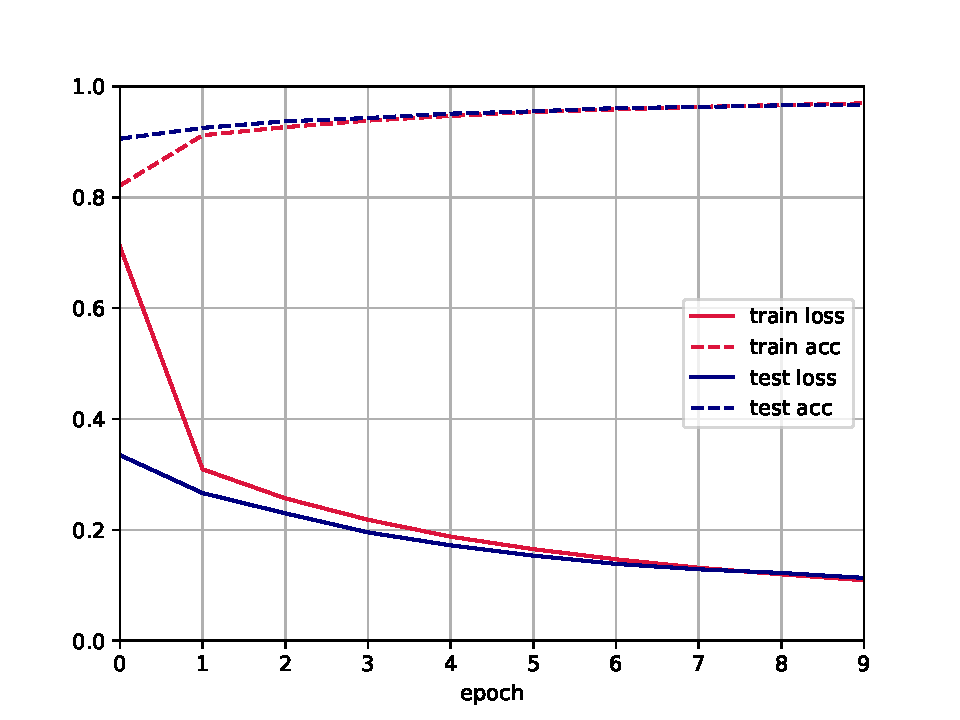
\includegraphics[]{loss_plot.pdf}
	\end{figure}

	\begin{part}{3}[Out of Distribution (OOD) Analysis]$\,$
		Now, let's evaluate the usefulness of the predictive uncertainties of our model for test data that are dissimilar to our training data. These test data points are called out of distribution (OOD) points. Report both the in and out distribution test accuracies of your model. In a couple of sentences, discuss what you notice about these accuracies.
	\end{part}

	We get a rather striking discrepancy in the accuracies: for the in distribution accuracy we get $99.63\%$, and for the out of distribution accuracy we get a flat $0.00\%$. This makes sense, since there's no way the model should be able to predict a $3$ if it's only training data was $1$s and $6$s. Any output which isn't $1$ or $6$ in the training stage would be heavily penalized, and so as a result the network probably learns to zero out those weights, leading to it never predicting $3$.

	\begin{part}{4}
		Now let us consider the implications of what we have seen.  First, just as in Homework 2, we want the predictive uncertainties from our models to help us distinguish in-distribution test data (test data that are similar to data on which we trained our model) and OOD test data.  Look at some examples in which the model expresses uncertainty about an in-distribution output and in which the model expresses uncertainty about an out-of-distribution output.  Characterize what you see.  In what ways are the uncertainties of the model useful, and in what ways are they not?  Do you think training multiple models and boostrapping, like you did in Homework 2, would help?  (You do not have to code anything, just discuss.)
	\end{part}

	In many real world examples, and with sufficiently complex models, the OOD accuracy discrepancy is probably a lot less; for example if you trained a network on faces of cats and dogs it might reasonably classify a fox as somewhere in between these two labels. Even in our case, it never fully classified a $3$ as exactly a $1$ or a $6$, but rather leaned toward one based on some metric of graphical similarity.

	I don't think training multiple models and bootstrapping would help in the case of neural networks, since a larger neural network usually could learn smaller models as sub-models of itself. Maybe training several networks with different architectures and selecting the best performing one to then fully train would be more effective.

	\begin{part}{5}
		Suppose the postal service was going to use your model to help automatically sort mail by zipcodes (a real use of AI systems).  They want to make sure that their system is safe against adversarial attacks.  Let us suppose that the model is relatively safe against software attacks, that is, appropriate security is in place such that the adversary cannot simply change the weights of a deployed model without someone noticing (in practice, this would be an important element).  Three scenarios, however, are of concern to them:
	\end{part}

	\begin{parts}
		\begin{part}{a}
			Hardware attack: Suppose the adversary has access to the
			scanner used to take pictures of the envelopes.  How might
			they be able to change the outputs of the model to their
			desired ones?  What safeguards might be possible, and what
			are their benefits and limitations/drawbacks?
		\end{part}

		By changing a particular camera to have some unnoticeable dead/colored pixels in a corner, this might escape manual inspection, however the AI might learn to associate these pixels strongly with some sort of adversarial training goal. This might be mitigated by incorporating blurring, dead pixels, randomly changing color, rotating, etc the training data so that the network is resilient to these changing.

		\begin{part}{b}
			Input attack: Suppose the adversary has access to the
			envelopes prior to scanning.  How might they be able to
			change the outputs of the model to their desired ones?
			What safeguards might be possible, and what are their
			benefits and limitations/drawbacks?
		\end{part}

		They might add some markings to the envelopes which causes the network to associate these markings with a particular target. As in the previous example, the main way to get around this is to expand the training data, including random marks, burns, and other conditions to the envelopes.

		\begin{part}{c}
			Social Engineering attack: Suppose that the adversary
			has access to the teams that will be maintaining and
			retraining the model.  How might they be able to change the
			outputs of the model to their desired ones?  What safeguards
			might be possible, and what are their benefits and
			limitations/drawbacks?
		\end{part}

		This is a lot harder to mitigate using software, since you might be able to convince the team to implement your nefarious goals. One way you could solve this would be to use an external testing dataset, which the team is not able to access, and test the model performance against this secret dataset before deploying it to the market.
	\end{parts}
\end{parts}

% \begin{enumerate}
% 	\item
% 	      % FDV: Expecting something along the lines of the uncertainty is between classes that are in-distribution e.g. a 1 that looks kind of like a 6, etc. but given something out of distribution, can be very certain.
%
% 	\item
% 	      \begin{enumerate}
% 		      % FDV: consider e.g. blurring the camera with some oil,
% 		      % changing the background surface, changing the focus, etc. 
% 		      % FDV: consider small changes that people can't tell change
% 		      % the number but it does for the machine
% 		      % FDV: same from s23 applies, e.g. a phishing attack to
% 		      % get the team to retrain on bad data 
% 	      \end{enumerate}
% 	      When you consider possible safeguards, think broadly: What might
% 	      be done in software (relates to Part 4 above)?  Regarding the
% 	      system integration and work environment overall?  You may find
% 	      it useful to explore how you can manipulate your model by
% 	      changing inputs, etc. but no coding is required for this
% 	      question.
%
% \end{enumerate}

\end{document}
